\documentclass[a4paper,12pt,twoside,openright,titlepage]{article}

%Additional packages
\usepackage[utf8]{inputenc}
\usepackage[T1]{fontenc}
\usepackage[dutch,english]{babel}
\usepackage{syntonly}
\usepackage[official]{eurosym}

% Handle images
%\usepackage[graphicx]
\usepackage{graphicx}
\graphicspath{ {./images/}{./styles/} }
\usepackage{float}
\usepackage{wrapfig}

% Handle URLs
\usepackage{xurl}
\usepackage{hyperref}
\hypersetup{colorlinks=true, linkcolor=blue, citecolor=blue, filecolor=blue, urlcolor=blue, pdftitle=, pdfauthor=, pdfsubject=, pdfkeywords=}

% Tables and listings
\usepackage{multirow,tabularx}
\usepackage[table]{xcolor} % Table colors
\usepackage{scrextend}
\addtokomafont{labelinglabel}{\sffamily}
\usepackage{listings}
\usepackage{adjustbox}

% Turn on indexing
\usepackage{imakeidx}
\makeindex[intoc]

% Define colors
\usepackage{color}
\definecolor{ashgrey}{rgb}{0.7, 0.75, 0.71}



% Listing style
\lstset{
  backgroundcolor=\color{ashgrey}, % choose the background color; you must add \usepackage{color} or \usepackage{xcolor}; should come as last argument
  rulecolor=\color{black},         % if not set, the frame-color may be changed on line-breaks within not-black text (e.g. comments (green here))
  frame=single,	                   % adds a frame around the code
  basicstyle=\ttfamily,  % the size of the fonts that are used for the code
  extendedchars=true,    % lets you use non-ASCII characters; for 8-bits encodings only, does not work with UTF-8
  breakatwhitespace=true, % sets if automatic breaks should only happen at whitespace
  breaklines=true,        % sets automatic line breaking
  keepspaces=true,        % keeps spaces in text, useful for keeping indentation of code (possibly needs columns=flexible)
  columns=fullflexible,	  % Make sure no extra spaces are added.
  showstringspaces=false, % if true show spaces in strings adding particular underscores
  showspaces=false        % show spaces everywhere adding particular underscores; it overrides 'showstringspaces'
}



% Uncomment for production
% \syntaxonly

% Style
\pagestyle{headings}

% Turn on indexing
\makeindex[intoc]

% Define title page
\author{D. Leeuw}
\title{Linux: Systeemdocumentatie}
\date{\today\\
\vfill
\raggedright
\copyright\ 2020-2025 Dennis Leeuw\\

%\begin{figure}

\includegraphics[width=0.3\textwidth]{CC-BY-SA-NC.png}
%\end{figure}

Dit werk is uitgegeven onder de Creative Commons BY-NC-SA Licentie en laat anderen toe het werk te kopi\"eren, distribueren, vertonen, op te voeren, en om afgeleid materiaal te maken, zolang de auteurs en uitgever worden vermeld als maker van het werk, het werk niet commercieel gebruikt wordt en afgeleide werken onder identieke voorwaarden worden verspreid.


}

% Document start
\begin{document}
\selectlanguage{dutch}

\maketitle

%%%%%%%%%%%%%%%%%%%
%%% Introductie %%%
%%%%%%%%%%%%%%%%%%%

%B% \frontmatter
\section{Over dit Document}
\subsection{Leerdoelen}
Na het bestuderen van dit document heeft de lezer kennis van:
\begin{itemize}
\item hoe er gebruik gemaakt kan worden van de aanwezige documentatie op het systeem
\item de commando's: man, info, apropos, locate, whatis
\end{itemize}

Dit document sluit aan op de volgende onderdelen van de LPI:
\begin{itemize}
\item LPI Linux Essentials 010-160 - 6.2.2 Using the Command Line to Get Help (weight: 2)
\end{itemize}


\subsection{Voorkennis}
Voor een goed begrip van dit document wordt er van de lezer verwacht dat die weet:
\begin{itemize}
\item wat de shell is
\end{itemize}


%%%%%%%%%%%%%%%%%
%%% De inhoud %%%
%%%%%%%%%%%%%%%%%
%%% \tableofcontents

%B% \mainmatter
% Requires: shell
% Provides: man, locate, info, apropos, whatis
\section{Linux documentatie}
Bijna elk linux-systeem is standaard voorzien van een uitgebreide set van documentatie. De
meeste documentatie bevat de man-pages. `man' is een afkorting voor Manual ofwel handleiding. Dat zal je vaker tegen
gaan komen dat commando's op een Linux en andere Unix-systemen afkortingen zijn. Het afkorten scheelt typen, wat
cruciaal was op de oude stugge toetsenborden van de PDP-systemen waarop Unix is ontworpen. Op deze toetsenborden kreeg
je zere vingers van het typen, dus alles dat typen bespaarde was meegenomen.

\section{man-pages}
\index{Manual pages!man-pages}
De op het systeem aanwezig help van een Unix-achtig systeem is te vinden in de man-pages. De online Manual is verdeeld
in hoofdstukken.

\begin{enumerate}
\item Executable programs or shell commands
\item System calls (functions provided by the kernel)
\item Library calls (functions within program libraries)
\item Special files (usually found in /dev)
\item File formats and conventions eg /etc/passwd
\item Games
\item Miscellaneous (including macro packages and conventions), e.g. man(7), groff(7)
\item System administration commands (usually only for root)
\item Kernel routines [Non standard]
\end{enumerate}

Voor gebruikers zijn de belangrijkste hoofdstukken die over de commando's gaan, 1 en 8, en die over de configuratie
bestanden 5. Om een beetje vertrouwd te raken met de man-pages gaan we de manual page over man bekijken. Type:

\begin{lstlisting}[language=bash]
$ man man
\end{lstlisting}

Met de pijltjes toetsten omhoog en naar beneden kan je door de pagina scrollen en met q verlaat je de manual-pagina.
Scrollend door de pagina kom je ook de hierboven al genoemde hoofdstuk indeling tegen. Verder kom je kopjes tegen met
hoofdletter. Veel voorkomende koppen zijn:

\begin{verbatim}
NAME: naam van het commando met een korte uitleg

SYNOPSIS: syntax van het commando

DESCRIPTION: een beschrijving van het commando

OPTIONS: welke opties kent het commando

EXAMPLES: voorbeelden hoe het commando te gebruiken

AUTHORS: wie heeft de manual-page geschreven

SEE ALSO: doorverwijzingen naar andere documentatie
\end{verbatim}

Om snel te zoeken naar bepaalde stukken in een manual-page kan je de / gebruiken. Als je een man-page open hebt staan en
je typt

\begin{lstlisting}[language=bash]
/EXAMPLES
\end{lstlisting}

en deze kop bestaat in de pagina dan kom je meteen bij de examples terecht. Snel door de man-pages scrollen kan door
gebruik te maken van PgUp en PgDn toetsen.


\section{Welk commando moet ik hebben?}
\begin{figure}

\includegraphics[width=0.4\linewidth]{linuxreader-img028.png}
	\caption{Het zoeken van informatie}
\end{figure}

Om uit te vinden welk commando je kan gebruiken om iets op het systeem te bereiken kan je man -k gebruiken. Een
alternatief commando is apropos. Type eens:

\begin{lstlisting}[language=bash]
$ apropos `make directories'
\end{lstlisting}
je vindt dan het `mkdir' commando. Het nadeel van dit zoek systeem is dat het redelijk specifiek is.

\begin{lstlisting}[language=bash]
$ apropos `make directory'
\end{lstlisting}
doet niets. Als je het dus niet meteen vindt probeer dan enkelvoud- en meervoudsvormen.

Heb je een commando gevonden waarvan je denkt dat het is wat je nodig hebt probeer dan man -f of whatis.

\begin{lstlisting}[language=bash]
$ whatis mkdir
\end{lstlisting}

Dit geeft een korte beschrijving van een commando en voor de volledige manual gebruiken we het man commando:
\begin{lstlisting}[language=bash]
$ man mkdir
\end{lstlisting}

Extra uitleg van een commando kan vaak ook gevonden worden door -h of --help aan het commando toe te voegen met een
spatie.

\begin{figure}[H]
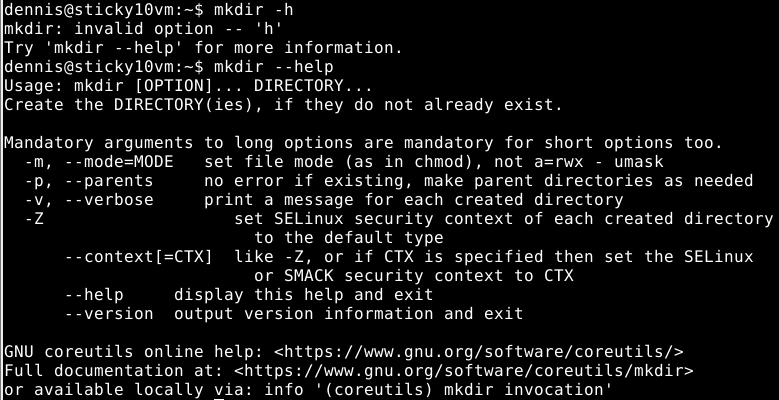
\includegraphics[width=0.8\linewidth]{linuxreader-img029.png}
	\label{fig:DocHelp}
	\caption{Gebruik van -h of --help}
\end{figure}

Zoals je ziet in \ref{fig:DocHelp} dat -h een error melding geeft en ons vertelt dat we -{}-help moeten gebruiken. Ook wordt er verteld wat we de
volledige documentatie online kunnen vinden in de info-documentatie.


\section{De opties -h en -{}-help}
Extra uitleg van een commando kan vaak ook gevonden worden door de optie -h of -{}-help aan het commando toe te voegen.

\begin{lstlisting}[language=bash]
$ mkdir -h
mkdir: invalid option -- 'h'
Try 'mkdir --help' for more information.
$ mkdir --help
Usage: mkdir [OPTION]... DIRECTORY...
Create the DIRECTORY(ies), if they do not already exist.

Mandatory arguments to long options are mandatory for short options too.
  -m, --mode=MODE   set file mode (as in chmod), not a=rwx - umask
  -p, --parents     no error if existing, make parent directories as needed,
                    with their file modes unaffected by any -m option.
  -v, --verbose     print a message for each created directory
  -Z                   set SELinux security context of each created directory
                         to the default type
      --context[=CTX]  like -Z, or if CTX is specified then set the SELinux
                         or SMACK security context to CTX
      --help        display this help and exit
      --version     output version information and exit

GNU coreutils online help: <https://www.gnu.org/software/coreutils/>
Full documentation <https://www.gnu.org/software/coreutils/mkdir>
or available locally via: info '(coreutils) mkdir invocation'
\end{lstlisting}

%\begin{figure}[H]
%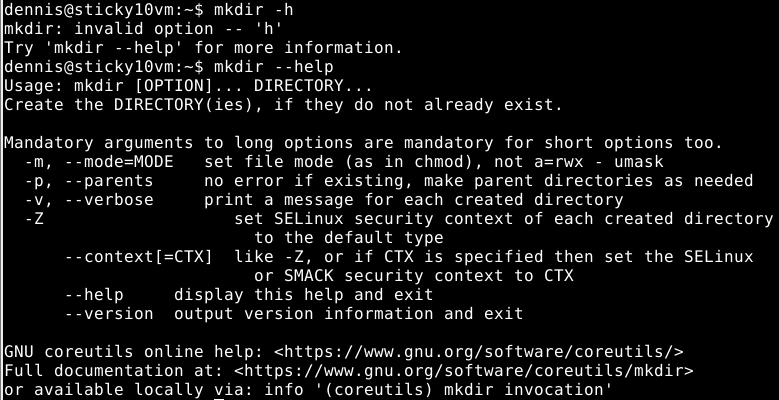
\includegraphics[width=0.8\linewidth]{linuxreader-img029.png}
%	\label{fig:DocHelp}
%	\caption{Gebruik van -h of --help}
%\end{figure}

In het voorgaande zie je dat -h een error melding geeft en ons vertelt dat we -{}-help moeten gebruiken. Ook wordt er verteld dat we de volledige documentatie kunnen vinden in de info-documentatie. Waarover later meer.


\section{Info}
The GNU-project heeft een eigen documentatie systeem ontworpen dat info genoemd wordt. Het is
een hypertext, dus met links, gerelateerd systeem. Dit is dus documentatie dat je naast man tegen komt op systemen.
Mocht je dus in man niet vinden wat je zoekt, misschien kan je dan eens info proberen. Ook in info werken de pijltjes
voor het scrollen en is q er weer om het systeem te verlaten. Een extra functie is de enter-toets die je kan gebruiken
om een link te volgen.

\section{/usr/share/doc}
Een andere plek waar we op ons systeem informatie kunnen vinden is in de /usr/share/doc directory. Met het commando `ls'
kan je een listing van een directory opvragen. Type

\begin{lstlisting}[language=bash]
$ ls /usr/share/doc
\end{lstlisting}

en een enorme lijst van directories vliegt over je scherm. Dit is de documentatie van elk pakket dat op het systeem
ge\"installeerd is. Een linux systeem is opgebouwd uit allerlei software pakketten die vanaf source code door de
distributie maker gecompileerd zijn. De informatie die met de source code meekwam, zoals de licentie-bestanden,
eventuele FAQ-bestanden, READMEs etc. die vind je terug in de subdirectories van /usr/share/doc. Belangrijk zijn vaak
de voorbeeld configuratie-bestanden.

\section{Internet}
Als laatste documentatie bron willen we graag het Internet vermelden. Omdat GNU/Linux een open source besturingssysteem is is er heel veel online te vinden. De kans dat jij als eerste tegen een probleem aanloopt is zeer klein. Het is dus naast de voornoemde bronnen \'e\'en van de eerste zaken om te raadplegen.

De broncode van alle software is openbaar en veel van de projecten hebben hun eigen website met vaak ook een eigen forum\index{forum} om contact te houden met gebruikers. Veel informatie is terug te vinden in de fora en de FAQs\index{FAQ}.


\section{Opdrachten}
\begin{itemize}
\item Welk hoofdstuk in de Linux Manual bevat een beschrijving van de door de normale gebruiker te gebruiken commando's?
\item Welk commando gebruik je om een manual-pagina te krijgen over het \texttt{rmdir} commando?
\item Hoe verlaat je een manual-pagina?
\item Als je wilt weten welk copyright er op \texttt{bash} zit, waar ga je dan zoeken op een Linux systeem?
\item Zoek in de manual page van \texttt{cat} naar EXAMPLES en kopieer de voorbeelden in je antwoord document.
\end{itemize}


%%%%%%%%%%%%%%%%%%%%%
%%% Index and End %%%
%%%%%%%%%%%%%%%%%%%%%
%B% \backmatter
\printindex

% End document
\end{document}
%%% Last line %%%
